\documentclass[conference, 10pt]{IEEEtran}

% ─── Packages ──────────────────────────────────────────────────────────────────
\usepackage[utf8]{inputenc}
\usepackage[T1]{fontenc}
\usepackage{amsmath, amssymb}
\usepackage{graphicx}
\usepackage{booktabs}
\usepackage{hyperref}
\usepackage{xcolor}
\usepackage{caption}
\usepackage{subcaption}
\usepackage{multirow}
\usepackage{url}
\usepackage{float}

\graphicspath{{figures/}}

% ─── Title ─────────────────────────────────────────────────────────────────────
\title{\LARGE Computer Vision -- Tasks 2-3:\\Ball Counting, Ball Detection and Table Retrieval\\with Deep Learning}

\author{
  \IEEEauthorblockN{João Proença, Joana Pimenta, Ricardo Ribeiro}
  \IEEEauthorblockA{M.IA | FEUP, 2025/2026}
}

\begin{document}
\maketitle

% ═══════════════════════════════════════════════════════════════════════════════
% INTRODUCTION
% ═══════════════════════════════════════════════════════════════════════════════

\section{Introduction}

This report presents three tasks related to pool ball analysis using deep learning techniques.
Task~2 addresses pool ball counting through CNN regression, Task~3a tackles pool ball detection, and Task~3b explores table retrieval, finding the most similar pool table configuration to a given query image.
Each task explores different computer vision paradigms, from image-level counting to object-level detection and content-based image retrieval.

% ═══════════════════════════════════════════════════════════════════════════════
% TASK 2 — POOL BALL COUNTING
% ═══════════════════════════════════════════════════════════════════════════════

\section{Task 2: Pool Ball Counting via CNN Regression}

\subsection{Problem Formulation}

Given an image of a pool table, the goal is to predict the number of balls visible on the table.
We formulate this as a \textbf{regression problem}, where a CNN backbone extracts visual features and a fully connected head outputs a single continuous value representing the ball count.

\subsection{Dataset}
We aggregate four COCO-format pool ball datasets from Roboflow Universe~\cite{ds_8ballpool, ds_poolbilliard, ds_poolballsdetection, ds_poolballdetection}.
The test set (20\%) is drawn exclusively from the original dataset; the remainder is split 80/20 into train/val.
To mitigate domain shift, the original dataset is oversampled 4$\times$ in the training pool.
Augmentations are applied on-the-fly and include random crop, horizontal/vertical flips, 360° rotation, perspective distortion, color jitter, random grayscale, and Gaussian blur.

\subsection{Model Architecture}

We evaluate five pretrained backbones, each modified for single-value regression output by replacing the classification head with a dropout layer ($p=0.3$) followed by a linear layer mapping to a single neuron:

\begin{itemize}
  \item \textbf{ResNet-18}~\cite{he2016resnet}
  \item \textbf{EfficientNet-B0}~\cite{tan2019efficientnet}
  \item \textbf{VGG-16}~\cite{simonyan2015vgg}
  \item \textbf{Inception v3}~\cite{szegedy2016inception}
  \item \textbf{MobileNet v3}~\cite{howard2019mobilenet}
\end{itemize}

\subsection{Training Setup}

All models are trained for 100 epochs using Adam~\cite{kingma2015adam} ($\text{lr}=10^{-4}$, weight decay~$=10^{-4}$) with the Huber loss~\cite{huber1964robust}.
A \texttt{ReduceLROnPlateau} scheduler (patience=5, factor=0.5) adapts the learning rate.
The best model is selected based on validation loss.
Input images are resized to $224 \times 224$ (or $299 \times 299$ for Inception~v3).

\subsection{Results}
Table~\ref{tab:task2_results} summarizes test set performance across all backbones.

\begin{table}[h]
\centering
\caption{Task 2 — Test set results across backbones.}
\label{tab:task2_results}
\begin{tabular}{lcccc}
\toprule
\textbf{Backbone} & \textbf{MAE}$\downarrow$ & \textbf{MSE}$\downarrow$ & \textbf{RMSE}$\downarrow$ & \textbf{Acc}$\uparrow$ \\
\midrule
ResNet-18             & 0.863 & 1.389 & 1.178 & 40.8\% \\
EfficientNet-B0       & 0.721 & 0.862 & 0.928 & 40.8\% \\
VGG-16                & 0.697 & 0.783 & 0.885 & 42.9\% \\
\textbf{Inception v3} & \textbf{0.627} & \textbf{0.676} & \textbf{0.822} & \textbf{53.1\%} \\
MobileNet v3          & 0.940 & 1.599 & 1.264 & 30.6\% \\
\bottomrule
\end{tabular}
\end{table}

Inception~v3 leads on all four test metrics, with VGG-16 as a close second.
MobileNet~v3 underperforms across the board, suggesting its lightweight architecture lacks the capacity to capture fine-grained spatial cues for counting.

Table~\ref{tab:task2_full} shows evaluation on the full original dataset, which includes training images.

\begin{table}[h]
\centering
\caption{Task 2 — Full original dataset evaluation.}
\label{tab:task2_full}
\begin{tabular}{lcccc}
\toprule
\textbf{Backbone} & \textbf{MAE}$\downarrow$ & \textbf{MSE}$\downarrow$ & \textbf{RMSE}$\downarrow$ & \textbf{Acc}$\uparrow$ \\
\midrule
ResNet-18             & 0.522 & 0.616 & 0.785 & 63.2\% \\
EfficientNet-B0       & 0.464 & 0.423 & 0.651 & 66.4\% \\
VGG-16                & 0.444 & 0.348 & 0.590 & 65.6\% \\
\textbf{Inception v3} & \textbf{0.297} & \textbf{0.195} & \textbf{0.442} & \textbf{82.6\%} \\
MobileNet v3          & 0.630 & 0.730 & 0.855 & 49.8\% \\
\bottomrule
\end{tabular}
\end{table}

Inception~v3 again leads across all metrics on the full original dataset, achieving 82.6\% accuracy and the lowest MAE (0.297), confirming that its strong test-set performance generalises well to the broader in-domain distribution.
VGG-16 and EfficientNet-B0 follow closely, while MobileNet~v3 remains the weakest.
Training convergence curves are provided in Appendix~\ref{app:training_curves}.

\subsection{Grad-CAM Analysis}
To understand where the model focuses during counting, we apply Grad-CAM~\cite{selvaraju2017gradcam} to the final convolutional layer of Inception~v3. Visualizations in Appendix~\ref{app:gradcam} show broad activations over the table surface, consistent with global spatial aggregation. In failure cases, activation spreads toward table edges, suggesting confusion with non-ball features


% ═══════════════════════════════════════════════════════════════════════════════
% TASK 3a — DETECTION
% ═══════════════════════════════════════════════════════════════════════════════

\section{Task 3a: Pool Ball Detection}

\subsection{Problem Formulation}

Given an image of a pool table, the goal is to localize and classify every ball with a bounding box.
We treat this as an \textbf{object detection problem} over a unified 4-class taxonomy --- \textit{Cue}, \textit{Solid}, \textit{Striped}, and \textit{Black} --- derived from the original 8-Ball Pool annotations (the \textit{Dot} table-spot class and the generic \textit{balls} supercategory are excluded).

\subsection{Dataset}

We reuse the same four Roboflow COCO datasets as Task~2~\cite{ds_8ballpool,ds_poolbilliard,ds_poolballsdetection,ds_poolballdetection}, remapping each source's native categories onto the shared 4-class taxonomy following the standard 8-ball convention: cue ball $\rightarrow$ \textit{Cue}, balls 1--7 $\rightarrow$ \textit{Solid}, ball 8 $\rightarrow$ \textit{Black}, balls 9--15 $\rightarrow$ \textit{Striped}; ambiguous categories (e.g.\ generic \textit{Object\_Ball}) are dropped.
A domain analysis reveals substantial covariate shift across sources (resolutions from $416\times416$ to $2200\times1295$, mean brightness 0.27--0.54, mean relative bbox area spanning an order of magnitude), motivating a controlled, progressive evaluation of how much auxiliary data helps.

\textbf{Split strategy.} The \textbf{test set} is fixed across all experiments: 20\% of the original dataset only (247 images), held out so every model is evaluated on the same in-domain distribution. Each experiment then splits its data pool 80/20 into train/val.

\subsection{Progressive Data Experiments}

To quantify the effect of adding out-of-domain data, we define four cumulative experiments, all evaluated on the same fixed test set:

\begin{itemize}
  \item \textbf{exp1 --- original only}: 8-Ball Pool training split.
  \item \textbf{exp2 --- + Pool Billiard}: adds all Pool Billiard splits.
  \item \textbf{exp3 --- + Pool Balls Detection}: further adds the v13 dataset.
  \item \textbf{exp4 --- all data}: further adds Pool Ball Detection v5.
\end{itemize}

\subsection{Models and Training Setup}

We finetune three detectors with complementary inductive biases:

\begin{itemize}
  \item \textbf{YOLOv8n}~\cite{jocher2023yolov8}: a one-stage anchor-free CNN detector, finetuned via \texttt{ultralytics} from COCO-pretrained weights for 50 epochs at $640\times640$, AdamW ($\text{lr}_0=10^{-4}$), with early stopping (patience~15) and built-in augmentation.
  \item \textbf{DETR}~\cite{carion2020detr} (\texttt{facebook/detr-resnet-50}): a transformer encoder--decoder using bipartite matching and a softmax no-object class.
  \item \textbf{Deformable DETR}~\cite{zhu2021deformabledetr} (\texttt{SenseTime/deformable-detr}): a sparse multi-scale deformable-attention variant using a sigmoid focal-loss head.
\end{itemize}

Both DETR-family models are finetuned for 100 epochs with the ResNet-50 backbone frozen, AdamW ($\text{lr}=10^{-5}$, weight decay $10^{-4}$), a cosine schedule, batch size~1, and inputs resized to a shortest edge of 800; the best checkpoint is selected on validation mAP@50.
Due to its restrictive computational cost, \textbf{Deformable DETR was only run for exp1 and exp2}.

\subsection{Evaluation Metrics}

We report \textbf{mAP@50}, \textbf{mAP@50:95}, \textbf{Precision}, and \textbf{Recall} (averaged over the four classes).

\subsection{Results}

Table~\ref{tab:task3a_results} reports the test-set performance of all model/experiment combinations.

\begin{table}[h]
\centering
\caption{Task 3a --- Pool ball detection test results. Best per model in bold; Deformable DETR was only trained on exp1--exp2.}
\label{tab:task3a_results}
\setlength{\tabcolsep}{4pt}
\begin{tabular}{llcccc}
\toprule
\textbf{Model} & \textbf{Exp} & \textbf{mAP@50}$\uparrow$ & \textbf{mAP@50:95}$\uparrow$ & \textbf{Prec}$\uparrow$ & \textbf{Rec}$\uparrow$ \\
\midrule
\multirow{4}{*}{YOLOv8n}
  & exp1 & 0.490 & 0.364 & 0.424 & 0.664 \\
  & exp2 & 0.783 & 0.592 & 0.746 & 0.761 \\
  & exp3 & 0.811 & 0.623 & 0.764 & 0.771 \\
  & \textbf{exp4} & \textbf{0.872} & \textbf{0.667} & \textbf{0.852} & \textbf{0.788} \\
\midrule
\multirow{4}{*}{DETR}
  & \textbf{exp1} & \textbf{0.076} & \textbf{0.048} & 0.083 & \textbf{0.200} \\
  & exp2 & 0.050 & 0.010 & 0.092 & 0.106 \\
  & exp3 & 0.056 & 0.012 & 0.077 & 0.137 \\
  & exp4 & 0.066 & 0.011 & \textbf{0.210} & 0.107 \\
\midrule
\multirow{2}{*}{Def.\ DETR}
  & exp1 & 0.229 & 0.182 & 0.284 & 0.293 \\
  & \textbf{exp2} & \textbf{0.626} & \textbf{0.503} & \textbf{0.789} & \textbf{0.624} \\
\bottomrule
\end{tabular}
\end{table}

\textbf{YOLOv8n} is the clear winner and the only model that benefits monotonically from added data: mAP@50 climbs from 0.490 (exp1) to 0.872 (exp4), the largest jump coming from Pool Billiard (exp1$\rightarrow$exp2, $+0.29$). Despite the domain shift, the auxiliary data acts as useful regularization for the CNN detector.
\textbf{Deformable DETR} also responds strongly, jumping from 0.229 to 0.626 mAP@50 between exp1 and exp2 and reaching a precision (0.789) competitive with YOLOv8n; its steep trajectory suggests further gains with exp3/exp4 data, left unexplored due to compute.
\textbf{Vanilla DETR} fails to converge in this low-data, small-object regime (mAP@50 $<0.08$ throughout, no benefit from added data), consistent with DETR's known need for long schedules and large datasets, compounded here by tiny ball sizes and a frozen backbone. Deformable DETR's multi-scale attention mitigates exactly these issues, explaining the large gap between the two transformers.

\textbf{Takeaway.} Under this data and compute budget, a lightweight pretrained CNN detector (YOLOv8n) substantially outperforms the transformers, and progressively adding heterogeneous auxiliary data yields the best result (mAP@50 $=0.872$). We use YOLOv8 rather than the latest YOLO releases, so an even stronger CNN baseline is likely attainable. With more compute, Deformable DETR could potentially close the gap, but YOLOv8n remains the best cost/performance trade-off here.

\subsection{Qualitative Comparison}

Figure~\ref{fig:yolo_def_detr} (Appendix~\ref{app:detection_compare}) overlays YOLOv8n (exp4) and Deformable DETR (exp2) predictions on shared test images against ground truth.
YOLOv8n produces tighter, more complete detections, whereas Deformable DETR misses small or occluded balls and is more prone to class confusions: it frequently mislabels the \textit{Cue} ball as \textit{Solid}/\textit{Striped} and even fires on table pockets, producing more detections than ground-truth balls (e.g.\ \texttt{compare\_03}). The shared samples make the recall gap (0.788 vs.\ 0.624) directly visible.

% ═══════════════════════════════════════════════════════════════════════════════
% TASK 3b — Table Retrieval
% ═══════════════════════════════════════════════════════════════════════════════

\section{Task 3b: Table Retrieval}

% TODO: Fill in Task 3b content here
\textit{[To be completed — Table Retrieval.]}

% ═══════════════════════════════════════════════════════════════════════════════
% CONCLUSION
% ═══════════════════════════════════════════════════════════════════════════════

\section{Conclusion}

% TODO: Write overall conclusion covering all tasks
\textit{[To be completed after all tasks are written.]}

% ═══════════════════════════════════════════════════════════════════════════════
% REFERENCES
% ═══════════════════════════════════════════════════════════════════════════════

\bibliographystyle{IEEEtran}
\bibliography{references}

% ═══════════════════════════════════════════════════════════════════════════════
% APPENDIX
% ═══════════════════════════════════════════════════════════════════════════════

\appendices

\section{Training Curves}
\label{app:training_curves}

Figures~\ref{fig:curve_loss}--\ref{fig:curve_acc} show the validation metrics across all five backbones over 100 training epochs.

\begin{figure}[H]
  \centering
  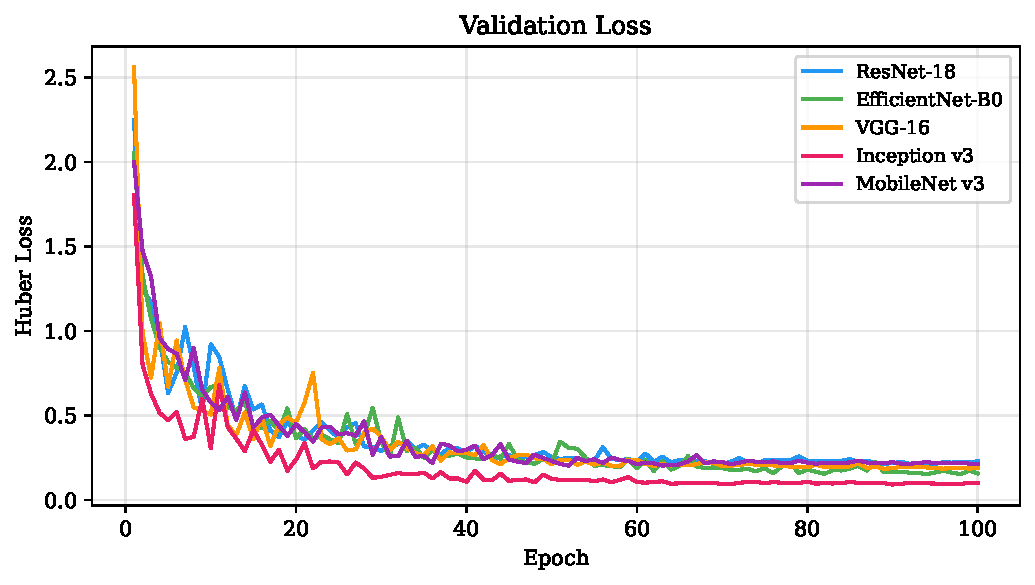
\includegraphics[width=\columnwidth]{training_curves/comparison_loss.pdf}
  \caption{Validation Huber loss across all backbones.}
  \label{fig:curve_loss}
\end{figure}

\begin{figure}[H]
  \centering
  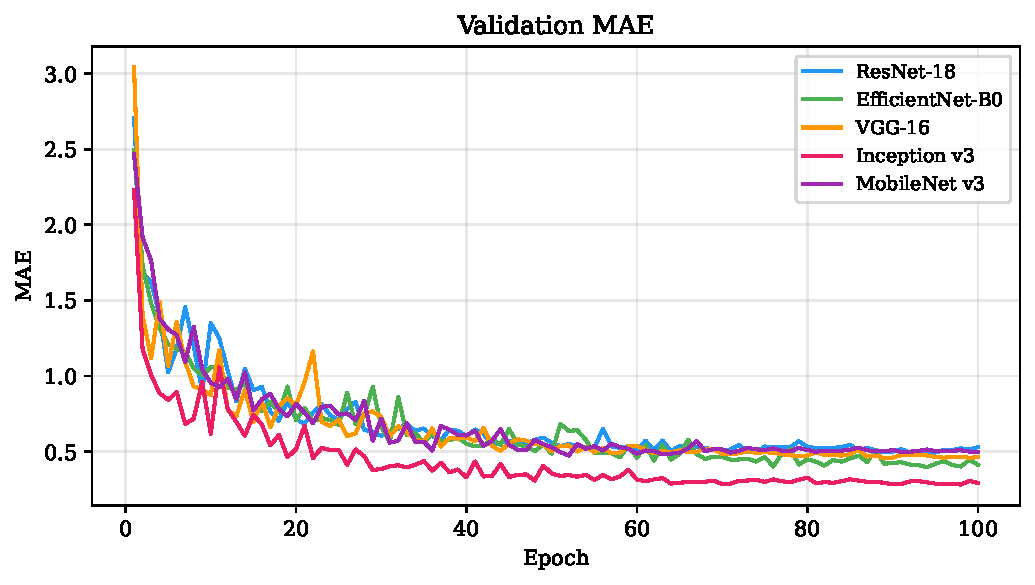
\includegraphics[width=\columnwidth]{training_curves/comparison_mae.pdf}
  \caption{Validation MAE across all backbones.}
  \label{fig:curve_mae}
\end{figure}

\begin{figure}[H]
  \centering
  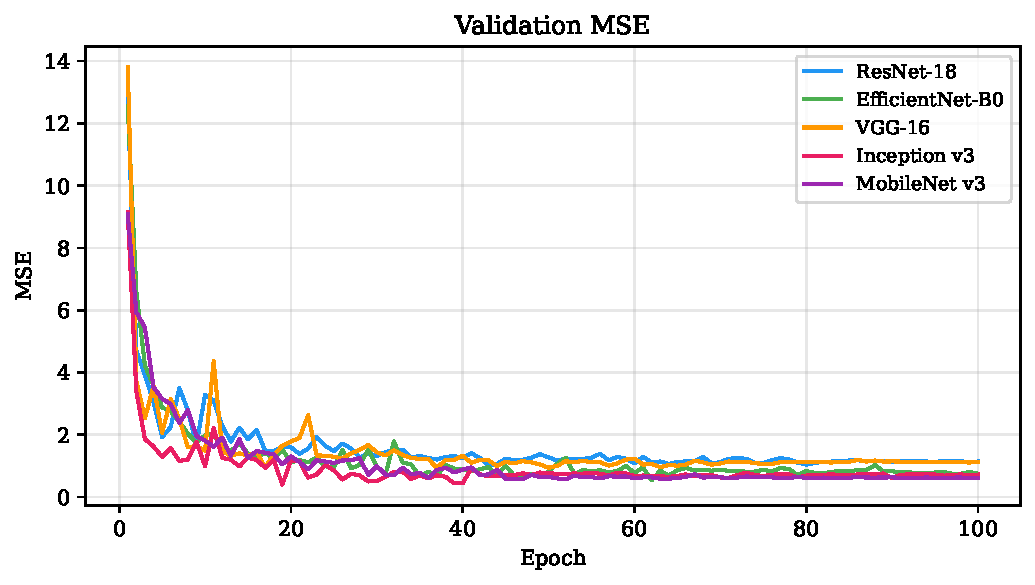
\includegraphics[width=\columnwidth]{training_curves/comparison_mse.pdf}
  \caption{Validation MSE across all backbones.}
  \label{fig:curve_mse}
\end{figure}

\begin{figure}[H]
  \centering
  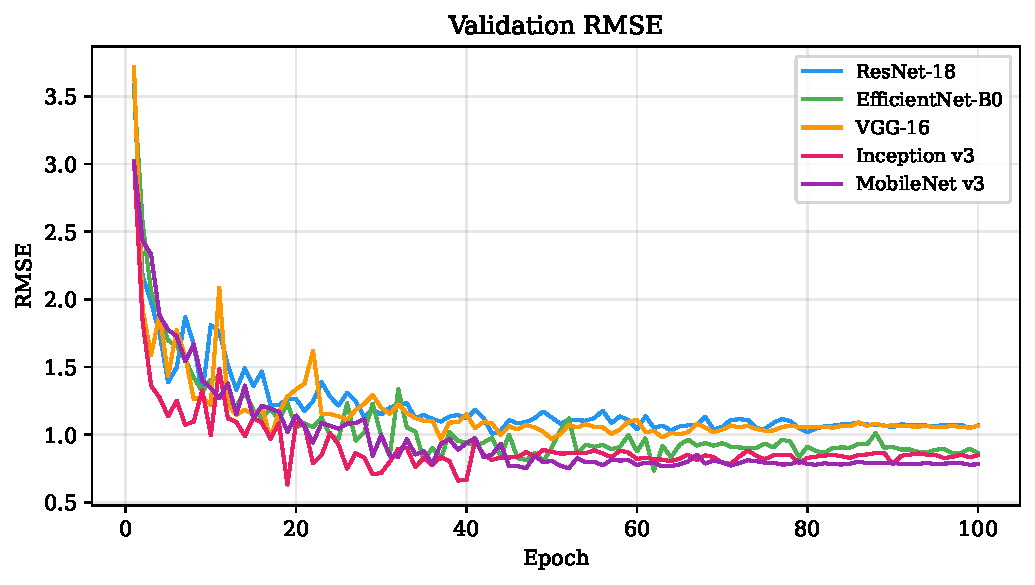
\includegraphics[width=\columnwidth]{training_curves/comparison_rmse.pdf}
  \caption{Validation RMSE across all backbones.}
  \label{fig:curve_rmse}
\end{figure}

\begin{figure}[H]
  \centering
  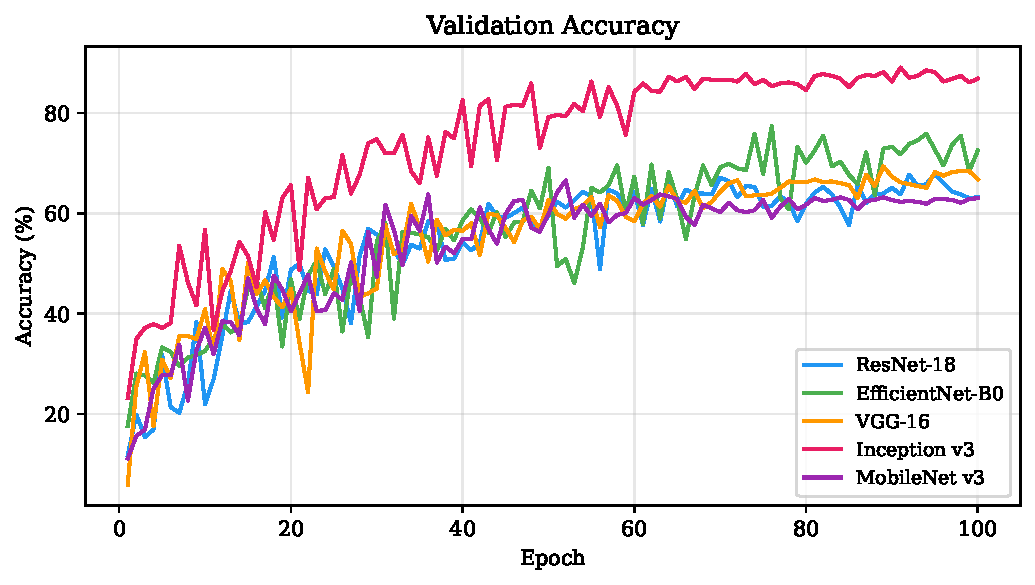
\includegraphics[width=\columnwidth]{training_curves/comparison_acc.pdf}
  \caption{Validation accuracy across all backbones.}
  \label{fig:curve_acc}
\end{figure}

\section{GradCAM Visualizations}
\label{app:gradcam}

Figure~\ref{fig:gradcam_inception} shows Grad-CAM heatmaps for Inception~v3 on three test set images (two correct predictions and one incorrect).
Each pair displays the original image (left) and the GradCAM overlay (right); ground truth and predicted ball counts are annotated in the image title.

\begin{figure}[H]
  \centering
  \begin{subfigure}[b]{\columnwidth}
    \centering
    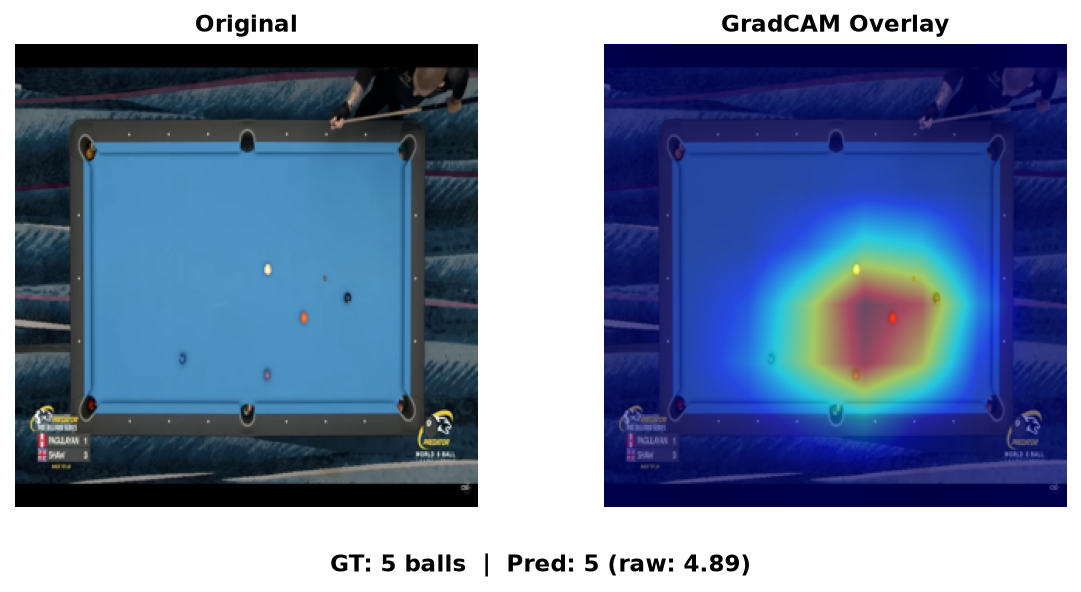
\includegraphics[width=0.95\columnwidth]{gradcam/inception_v3_00.png}
    \caption{Sample 1.}
  \end{subfigure}

  \vspace{0.3em}

  \begin{subfigure}[b]{\columnwidth}
    \centering
    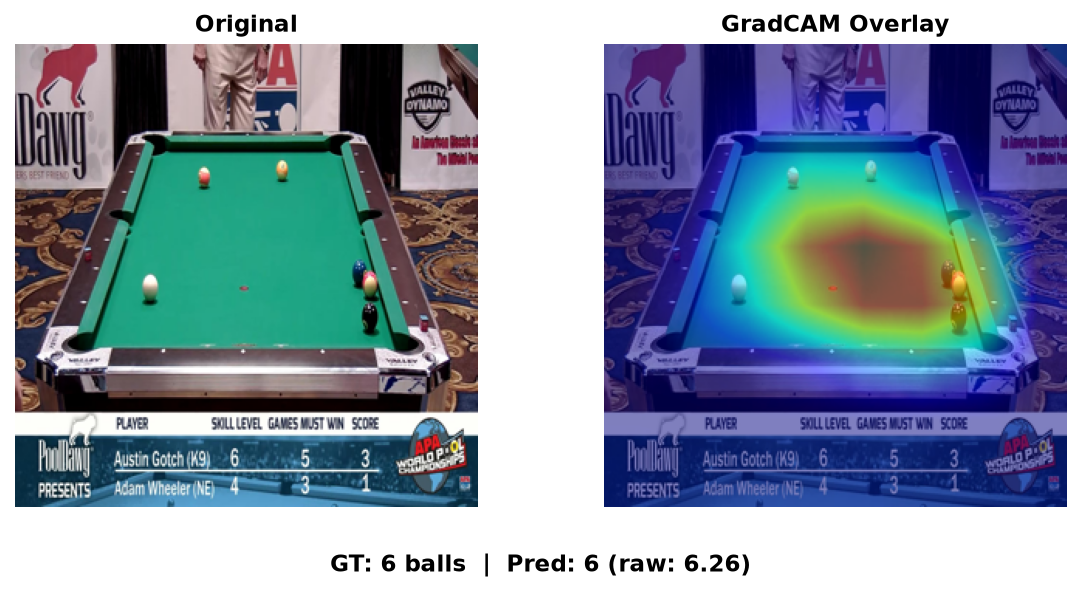
\includegraphics[width=0.95\columnwidth]{gradcam/inception_v3_01.png}
    \caption{Sample 2.}
  \end{subfigure}

  \vspace{0.3em}

  \begin{subfigure}[b]{\columnwidth}
    \centering
    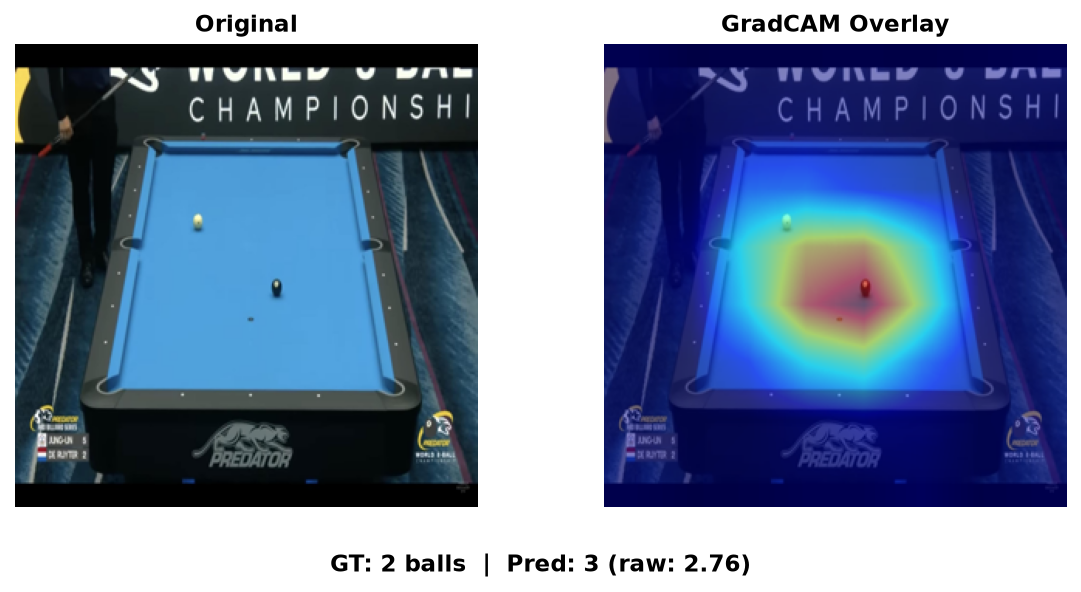
\includegraphics[width=0.95\columnwidth]{gradcam/inception_v3_02.png}
    \caption{Sample 3.}
  \end{subfigure}

  \caption{Inception v3 Grad-CAM visualizations on original test set images.}
  \label{fig:gradcam_inception}
\end{figure}

\section{Detection Comparison: YOLOv8n vs.\ Deformable DETR}
\label{app:detection_compare}

Figure~\ref{fig:yolo_def_detr} overlays the predictions of YOLOv8n (exp4) and Deformable DETR (exp2) on the same held-out test images, alongside the ground-truth boxes (green dashed).

\begin{figure}[H]
  \centering
  \begin{subfigure}[b]{\columnwidth}
    \centering
    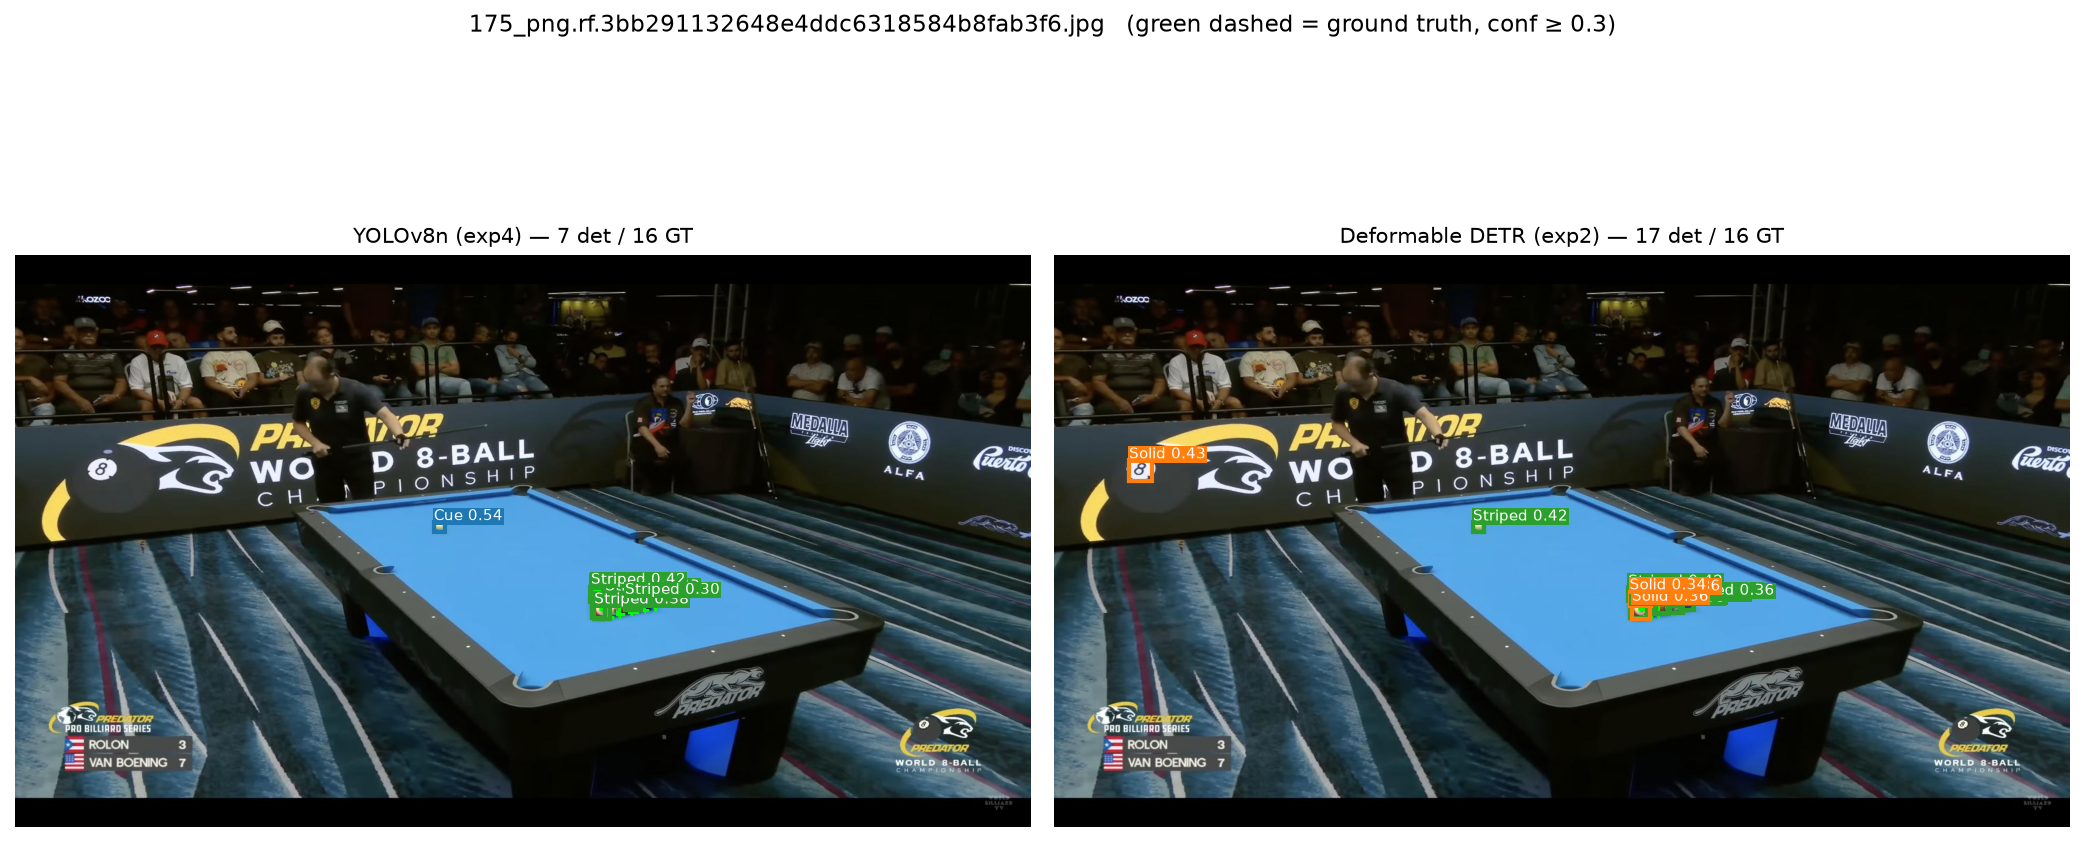
\includegraphics[width=\columnwidth]{yolo_def_detr/compare_00.png}
    \caption{Sample 1.}
  \end{subfigure}

  \vspace{0.3em}

  \begin{subfigure}[b]{\columnwidth}
    \centering
    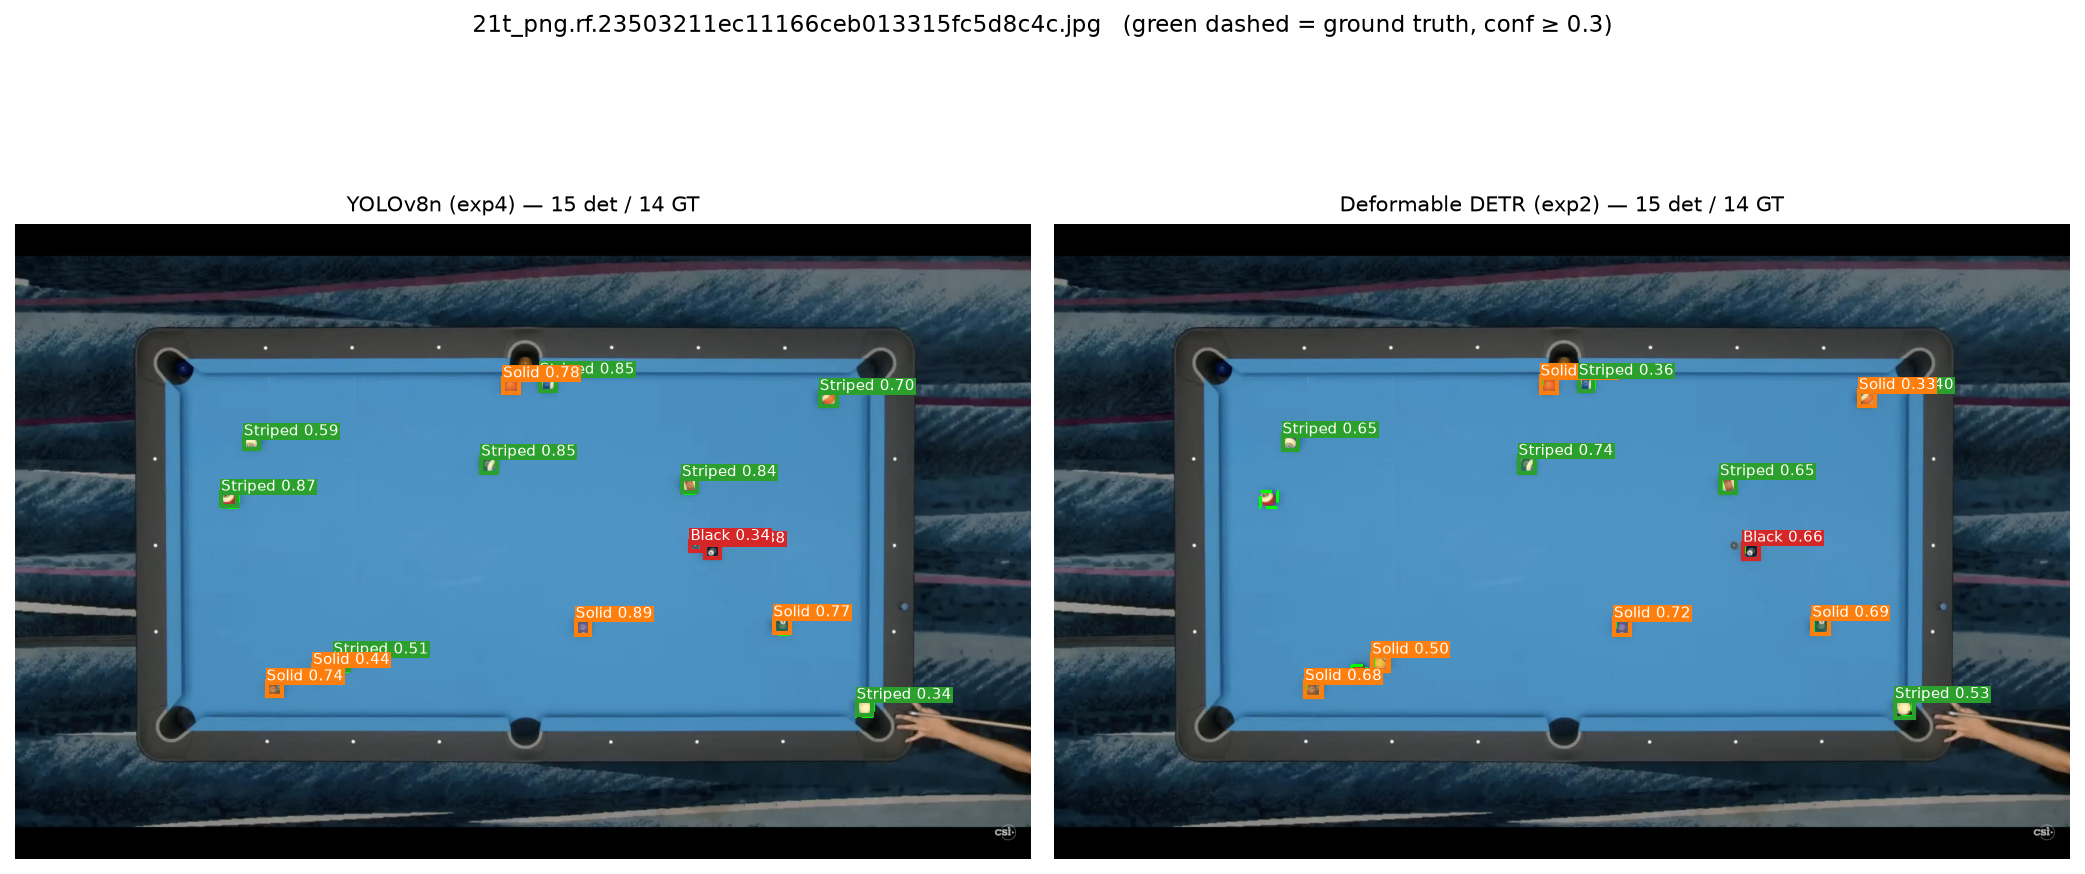
\includegraphics[width=\columnwidth]{yolo_def_detr/compare_01.png}
    \caption{Sample 2.}
  \end{subfigure}

  \vspace{0.3em}

  \begin{subfigure}[b]{\columnwidth}
    \centering
    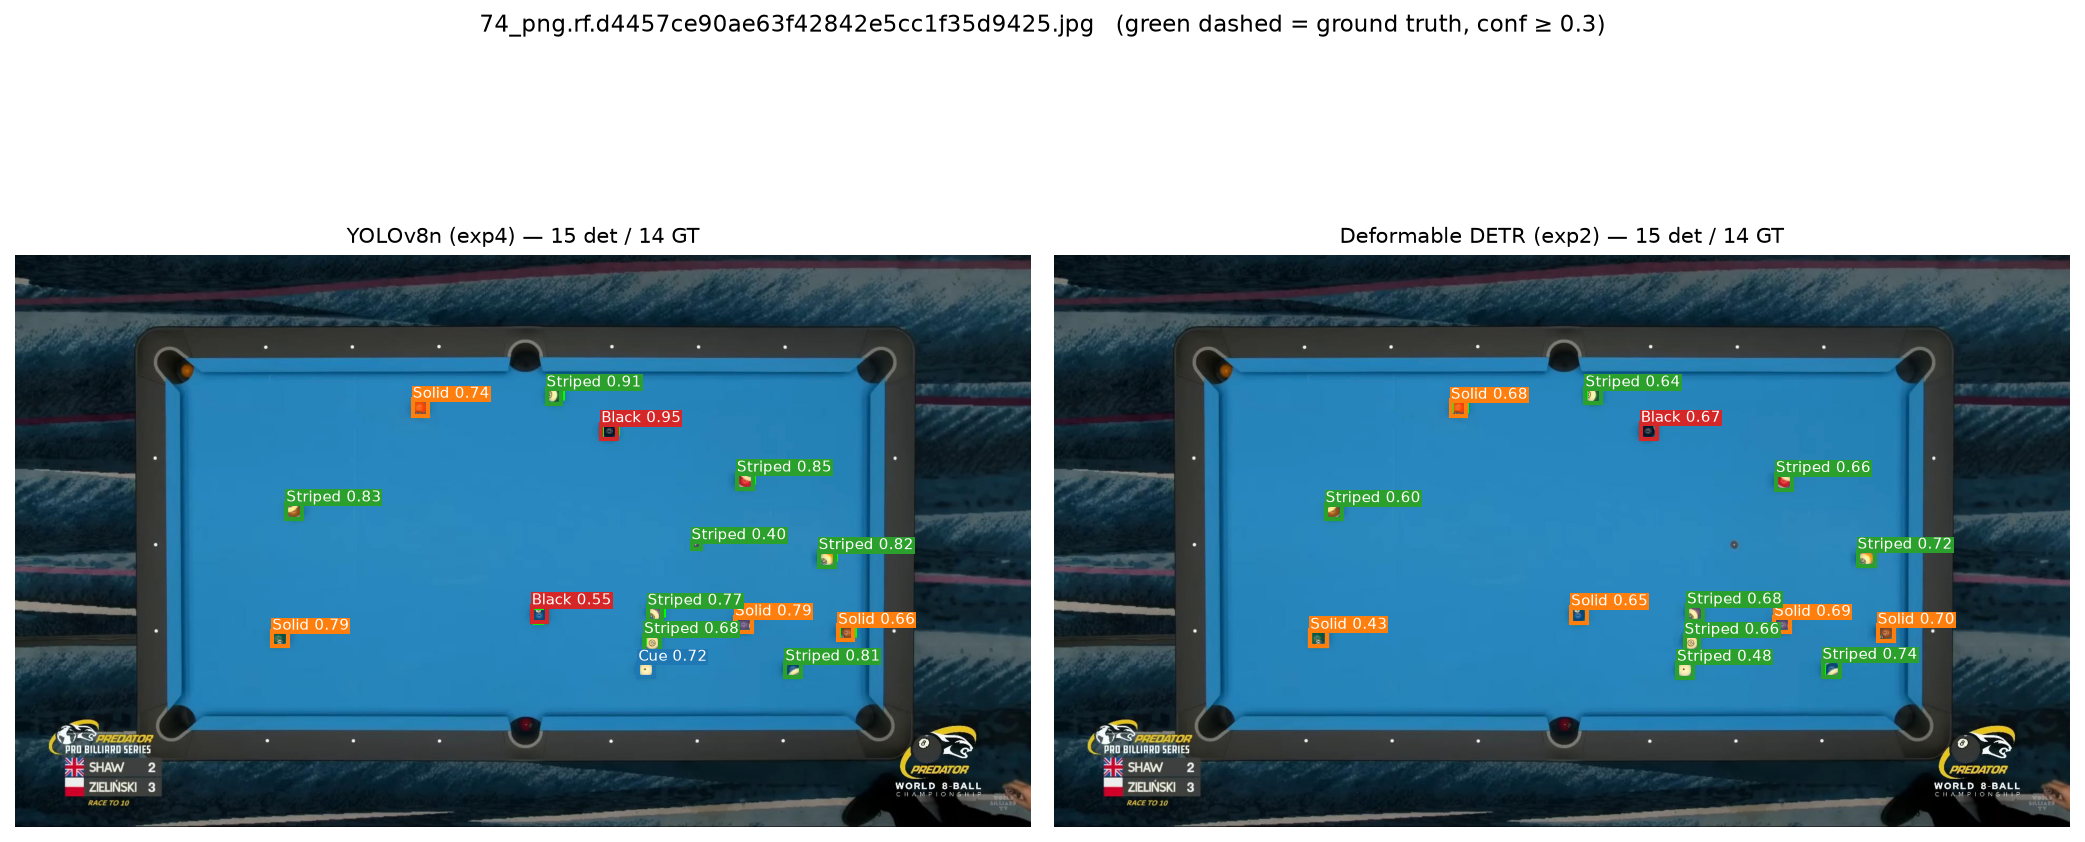
\includegraphics[width=\columnwidth]{yolo_def_detr/compare_02.png}
    \caption{Sample 3.}
  \end{subfigure}

  \vspace{0.3em}

  \begin{subfigure}[b]{\columnwidth}
    \centering
    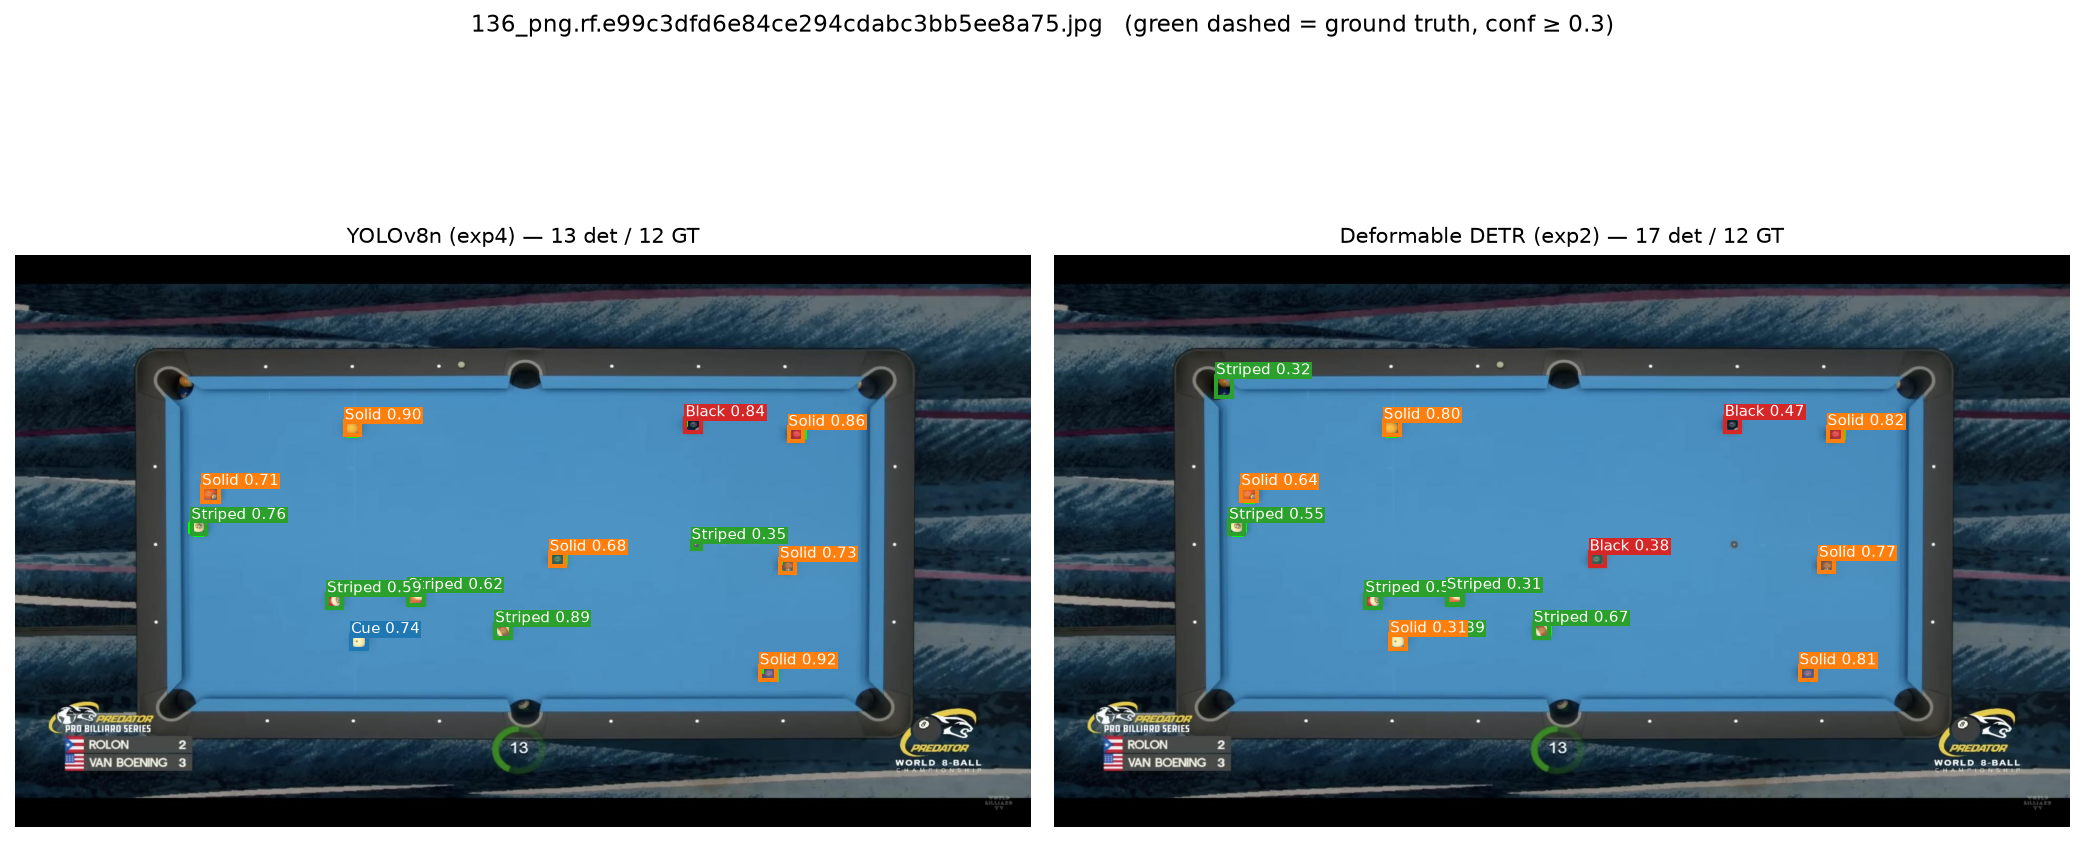
\includegraphics[width=\columnwidth]{yolo_def_detr/compare_03.png}
    \caption{Sample 4.}
  \end{subfigure}

  \caption{Qualitative detection comparison on shared test images: YOLOv8n (exp4, left) vs.\ Deformable DETR (exp2, right). Green dashed boxes are ground truth; colored solid boxes are model predictions with confidence scores.}
  \label{fig:yolo_def_detr}
\end{figure}

\end{document}